\section{项目的主要内容和技术路线}

\subsection{主要研究内容}

本研究尝试解决现有的处理器瞬态执行漏洞测试程序生成框架存在的四个问题。\par

第一个问题是瞬态执行漏洞的威胁模型和上下文环境是多样化的\cite{kocher2020spectre}\cite{horn2018meltdown}\cite{ragab2021rage}\cite{van2006cacheout},无论是用户态程序还是内核程序都有可能成为瞬态攻击的攻击者或者受害者,且各类 CPU 设置,诸如页表设置\cite{horn2018meltdown}、特权寄存器设置、飞地设置\cite{van2018foreshadow}、缓冲区设置\cite{moghimi2020medusa}等也会影响瞬态执行漏洞的执行。因此本测试程序生成框架需要提供足够多的环境初始化配置,以支持测试程序可以在不同的威胁模型和上下文环境中工作,进而挖掘出不同场景下的瞬态执行漏洞。\par

第二个问题在于现有的生成框架往往旨在生成一个完整的瞬态攻击漏洞利用程序,无论是直接随机生成还是分阶段随机生成,都是以整个程序为单位进行生成的,生成效率较为低下。但通过观察瞬态攻击的样例\cite{riscv-test}可以发现,一个完整的瞬态攻击漏洞利用程序根据其功能语义可以划分为多个阶段,且各阶段之间保持了一定程度的独立性,这为各阶段进行独立的指令生成和功能验证提供了可能。因此研究者有时可以仅对感兴趣的阶段和其强相关阶段进行指令生成,其余部分独立性较强的阶段则可以套用已有的模板,而无需重复进行随机生成;或者弱相关的阶段之间也可以分别独立生成,并在分别测试正确性后尝试组合拼接,进而实现完整攻击。本工作将对瞬态漏洞利用程序各阶段进行更细粒度的划分,尝试构造关联度尽可能低的阶段块。\par

第三个问题是现有的生成框架生成的指令序列缺乏语义信息。瞬态攻击程序的执行的各个阶段都有其语义和功能特性。但是常规的瞬态执行漏洞 Fuzzing 工作的测试程序生成器往往采用纯随机的指令生成策略\cite{oleksenko2022revizor}\cite{hur2022specdoctor},导致这类生成策略验证效率极其低下。如vanilla2 工具花费 50 hour 仅能找到一个 Meltdown 类型的漏洞\cite{hur2022specdoctor}。而SpecDoctor\cite{hur2022specdoctor}虽然对测试程序的三个阶段分别进行代码生成,但每个阶段总体上还是采用了纯随机的生成策略,并没有充分利用当前阶段的语义信息。本工作将尝试挖掘各阶段的语义信息,并利用语义信息指导该阶段测试程序生成,以期提高测试程序的有效性和瞬态执行漏洞挖掘的效率。\par

第四个问题在于现有的生成框架的随机指令生成策略\cite{hur2021difuzzrtl}会产生随机的控制转移指令和异常触发指令。前者会导致测试程序利用率降低,大量有效测试点被随机控制转移指令跳过\cite{soltcascade}。而后者会导致测试程序因为随机的异常事件提前结束,无法有效执行。因此本测试程序生成框架需要对控制转移指令和异常指令的生成加以引导、约束和排查,防止上述问题发生。\par

\subsection{技术路线}

从上述问题中可以看到,构建瞬态执行漏洞测试程序生成框架需要考虑以下几个方面:首先,测试程序生成器应该能够灵活地配置测试程序参数和运行环境,例如寄存器初始化、页表初始化、内存布局等,从而适配不同威胁模型和上下文的需求。其次,测试程序生成器需要能根据瞬态执行漏洞的特点,高效地生成瞬态漏洞触发程序,且程序应保持多样性和复杂性,以期触发不同类型的瞬态漏洞。最后,生成器需要能和其他验证工具,例如仿真器、硬件插桩工具、异常检测机制等协同工作。\par

为了弥补现有测试程序生成框架的缺陷和满足上述需求,我们提出了新的测试程序生成框架主要流程,如图\ref{review:frame}所示。我们使用两个 hjson 配置文件设置生成框架的生成参数,以决定测试程序的运行模式、内存分布、各类权重、寄存器初始值等,适配不同的威胁模型和上下文。然后我们的测试框架根据各内存区域、瞬态执行漏洞触发程序各阶段不同的功能特点和语义信息,有针对性地设置生成策略并产生汇编代码,然后根据内存布局配置、阶段语义等信息将各部分生成的汇编代码组装整合得到完整的测试程序,从而提高触发瞬态执行漏洞的成功率。最后对生成的程序用模拟器进行预执行,提前过滤掉明显不满足瞬态漏洞攻击要求的程序。\par

\begin{figure}[!h]
    \centering
    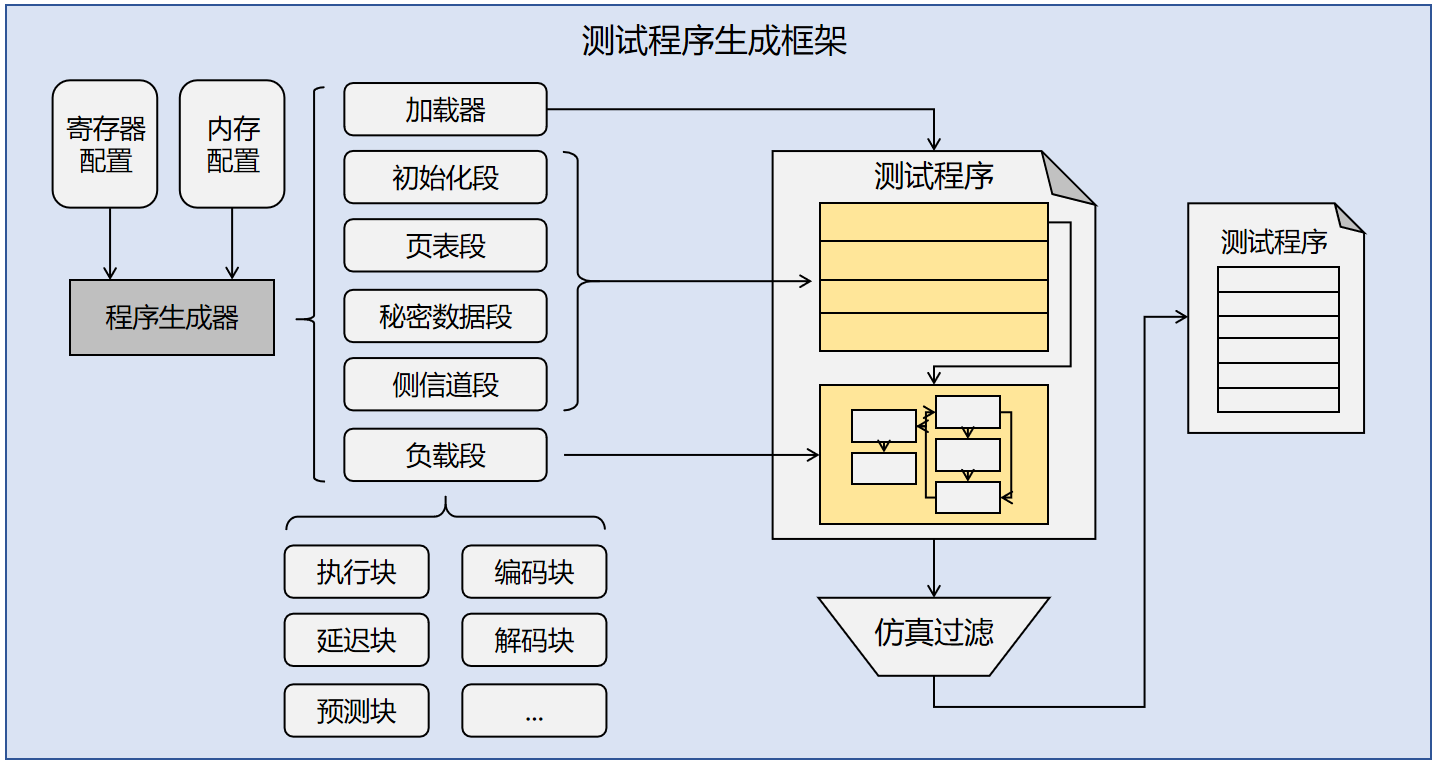
\includegraphics[width=\linewidth]
    {figure/proposal/generation-frame.png}
    \caption{测试程序生成框架}
    \label{review:frame}
\end{figure}

之后我们还会将测试程序生成框架和其他处理器差分测试框架进行集成,对一些开源处理器的瞬态执行漏洞进行挖掘,并与现有工作进行对比实验来验证该测试程序生成框架的效果。\par

针对上文中我们介绍的处理器瞬态执行漏洞测试程序生成框架的需求和现有框架存在的问题,我们将逐一介绍对应的五种解决方法及其技术细节。\par

\subsubsection{环境配置与初始化}

测试程序生成框架的参数配置包括两大类:1)威胁模型和上下文相关的参数,如寄存器的初始值、运行的特权级、是否启用虚拟地址、页表权限设置、内存功能布局等;2)测试程序生成策略相关的参数,如测试程序各阶段指令的生成策略、参数权重、是否套用模板等。我们将这些参数配置保存到 reg\_init.hjson 和 mem\_init.hjson 两个配置文件中。测试程序生成框架的使用者可以通过修改这两个配置文件,轻松改变实验的威胁模型和上下文环境,以及采取不同的测试程序生成策略。\par

\subsubsection{测试程序功能块划分}

我们通过观察瞬态攻击案例和总结相关工作,根据测试程序各个阶段的功能和语义,将测试程序划分为多个相对独立的功能块,具体如图\ref{review:block-partition}所示,后续根据实验需要还会对各功能块进行适当调整:\par

1. 初始化块 init:对执行环境进行初始化\par
2. 异常块 trap:处理程序执行时发生的异常\par
3. 延迟块 delay:延迟 predict 块得到源数据,迫使 predict 块进行预测\par
4. 预测块 predict:能发生预测执行的代码块,如果预测错误就会触发瞬态执行窗口,执行 encode 块的攻击代码\par
5. 执行块 runtime:调用瞬态漏洞训练和攻击的代码块,训练 predict 块预测错误,引发瞬态执行窗口\par
6. 返回块 return:predict 块预测正确时执行的无害代码\par
7. 编码块 encode:瞬态窗口中执行的有害代码,负责将机密数据泄露进侧信道\par
8. 解码块 decode:负责从侧信道还原机密数据\par
9. 退出块 exit:负责输出测试结果并结束测试程序\par

\begin{figure}[!h]
    \centering
    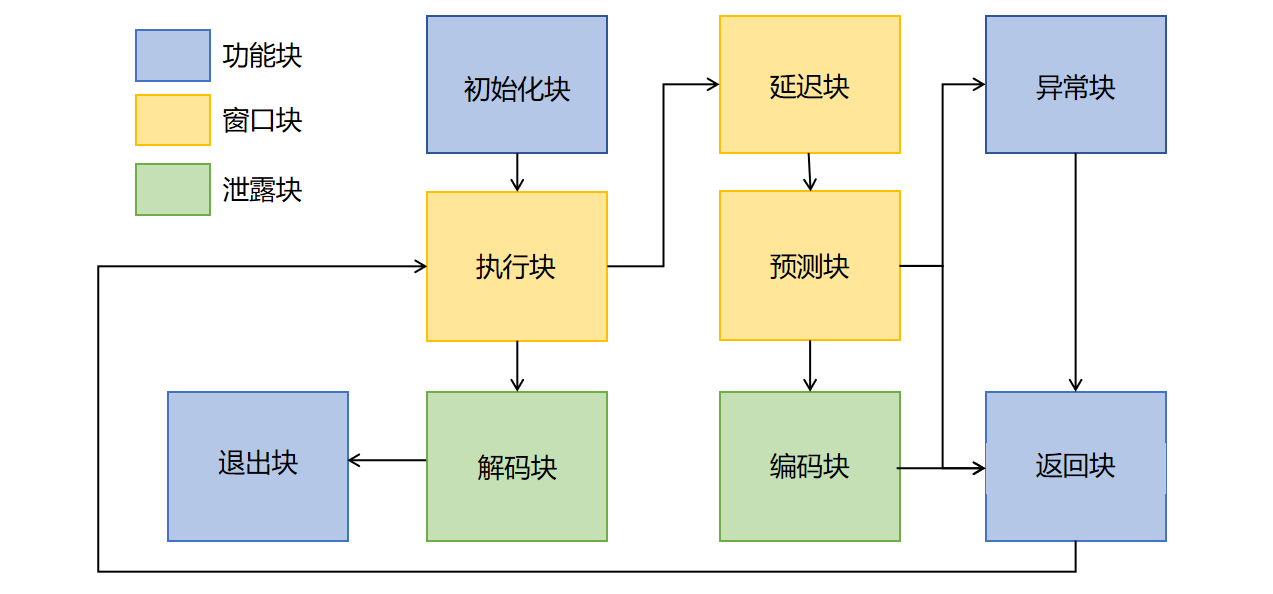
\includegraphics[width=\linewidth]{figure/proposal/block-partition.png}
    \caption{测试程序阶段划分}
    \label{review:block-partition}
\end{figure}

其中 init、trap、return、exit 四个代码块预先给定,是测试程序功能单元,称为功能块;runtime、delay、predict 块相互协作,负责瞬态窗口的触发,称为窗口块;encode、decode 块相互协作负责构建侧信道泄露数据,称为泄露块。其中功能块、窗口块、泄露块之间保持较高的独立性,相互之间功能影响较小。因此,我们可以重用验证生效的窗口块内容仅生成泄露块,也可以重用验证生效的泄露块仅生成窗口块,或者将独立测试得到的泄露块和窗口块两两组合,验证攻击的有效性。\par

通过分阶段测试程序生成,而不是一次随机生成完整瞬态漏洞攻击,可以降低单次有效测试程序生成的难度,提高有效测试程序生成的效率。

\subsubsection{各功能块基于语义生成}

不同于Revixor\cite{oleksenko2022revizor}等工作的纯随机指令生成方式,我们的测试生成框架对于每个代码块都将根据其语义和功能特征采取有针对性的生成策略,试图提高有效测试的生成效率。\par

如 delay 块主要依靠数据竞争、结构竞争产生延迟\cite{riscv-test},因此可以尝试让延迟块大概率生成乘除法指令、浮点指令等多周期指令,并让指令之间尽可能多的存在数据依赖,从而利用数据竞争、结构竞争产生足够的数据流延迟,迫使 predict 块执行预测执行并能打开足够大的瞬态窗口;对于 predict 块,可以根据 BOOM\cite{celio2017boomv2}、CVA6\cite{zaruba2019cost}等 RISCV 开源处理器预测执行的硬件逻辑总结出会预测执行的指令类型,并分别构建与 delay 块配合执行的代码模板,在这些模板的基础上加以突变,从而尝试提高生成代码触发瞬态窗口的概率;其他功能块也依各自特点制定生成策略。\par

另外每个代码都提供一个验证生效的默认模板代码,当测试程序考虑仅生成指定部分的代码块时,其余代码块可以简单采用默认模板代码,便于分阶段生成测试程序。

\subsubsection{控制流约束}

为了瞬态漏洞攻击可以执行成功,我们需要测试程序按照指定次序执行各个功能块。为了防止随机生成策略产生随机的控制流,使得瞬态执行漏洞攻击失败,我们需要对程序中的控制流进行约束,确保功能块按照指定次序顺利执行。\par

我们为每个功能块事先指定入口和出口,以及功能块间出口、入口的转移关系,例如 delay 块的出口抵达 predict 块的入口、runtime 块的出口抵达 decode 块的入口等。每个代码块的出口,我们根据场景提供 jump、branch、except 等转移指令,并根据跳转地址为这些指令生成配合使用的立即数。而在代码块内部,我们也会对控制流进行约束,例如通过首先生成数据流块,然后在数据流块之间提供确定的控制流转移等方法,确保代码块控制流可以从指定入口进入、指定出口退出。\par

\subsubsection{模拟器过滤}

虽然我们很小心的约束控制流和生成代码块,但是仍然可能会产生不满足测试需求的代码。比如随机的内存访问指令可能会在非瞬态窗口访问 secret 代码,或者 decode 产生的随机指令会触发异常,前者违反了瞬态漏洞攻击的执行规则,而后者会导致瞬态漏洞攻击执行失败,将这些程序交给后端处理器进行漏洞挖掘是没有意义。所以我们可以使用一个模拟器预执行这些程序,如果发现其存在上述问题则提前过滤,节约后端处理器仿真的时间。

\subsection{可行性分析}

SpecDoctor\cite{hur2022specdoctor}的工作已经证明分阶段代码生成是有效果,它通过三阶段代码的方式获得了远高于 vanilla1、vanilla2 等工作的性能。我们在其阶段分割的基础上,参考了常见的 Meltdown、Sepctre瞬态漏洞的代码案例,对瞬态漏洞程序进行了进一步的功能分割,从原来的三阶段细化为了 9 个功能块,使得代码的生成更加细粒度。且与原来的纯随机指令生成相比,我们基于语义的指令生成策略虽然在一定程度上会错过一些未知的 bug,但是对于相似结构的漏洞可以进行快速复现\cite{moghimi2020medusa}\cite{xiao2019speechminer},并比较高效地找到变种,而对于难以进行语义描述的功能块也可以采用纯随机的策略进行保底,故而漏洞挖掘的效率可以高于纯随机的生成方式。\par

通过使用 Verilator\cite{snyder2013verilator}等 RTL 模拟器,我们可以在 CVA6、BOOM 等开源 RISCV 处理器上模拟运行我们生成的测试程序,并根据瞬态漏洞触发情况及时检测生成策略的效率,指导我们调整生成策略。通过控制流约束的方法相较于随机指令生成,也可以大大提高生成程序的执行覆盖率\cite{soltcascade},提高触发瞬态漏洞的概率。\par

对于执行环境配置问题,我们通过分析已有的瞬态漏洞类型和 RISCV 处理器权限管理\cite{watermanrisc}的特点,总结了一系列威胁模型相关的特权寄存器、需要被初始化的寄存器组以及页表设置,我们从中抽象出必要的配置选项,并编写对应的初始化模块,即可满足多样化的威胁模型和上下文需求。\par

对于汇编指令级生成和模拟器过滤等,我们则可以使用一些开源的汇编指令生成工具如 razzle\cite{razzle}等进行汇编指令的生成,使用开源的模拟器比如 spike\cite{riscv-isa-sim}进行程序的预执行过滤,并根据需要进行代码修改和定制化处理。开源工具的存在,将大大减轻这部分辅助工作的工作量,使我们将重心放在瞬态漏洞测试程序生成策略的制定上。\par
